%%%%%%%%%%%%%%%%%%%%%%%%%%%%%%%%%%%%%%%%%%%%%%%%%%%%%%%%%%%%%%%%%
%2345678901234567890123456789012345678901234567890123456789012345
%        1         2         3         4         5         6     
\chapter{ICR optimization control}
\label{cha:ICR}
The implementation of the by GPs augmented MPC scheme is made up of three major steps.
First, MPC and GPs are conceptionally combined in an augmented MPC scheme in \cref{sec:augmentedcontroller}.
Second, a linear model for the prediction was derived in \cref{sec:predictionmodel}.
Third, in \cref{sec:software} the software used for the implementation is highlighted.

In this chapter the time-dependency is not explicitly written due to better readability.
%%%%%%%%%%%%%%%%%%%%%%%%%%%%%%%%%%%%%%%%%%%%%%%%%%%%%%%%%%%%%%%%%%%%%%%%%%%%%%%%%%%%%%%%%%%%%%%%%%%%%%%%%%%%%%%%%%%%%%%%%%%%%%%%%%%%%%%%%%%%%%%%%

\section{Augmented controller}
\label{sec:augmentedcontroller}
The purpose of the augmentation is to control a nonlinear process \eqref{eq:xdotnl} with a MPC scheme based on a linear prediction model \eqref{eq:xdotlin}.
\begin{align}
\dot{\mathbf{x}}_{nl} &= f \left( \mathbf{x},\mathbf{u},\mathbf{d} \right) \label{eq:xdotnl},\\
\dot{\mathbf{x}}_{lin} &= A \left( \mathbf{d} \right) \mathbf{x} + B \left( \mathbf{d} \right) \mathbf{u} + C \left( \mathbf{d} \right). \label{eq:xdotlin}
\end{align}
$\mathbf{x}$ denotes the states, $\mathbf{u}$ the inputs and $\mathbf{d}$ the disturbance variables which are treated as parameters.
The linear model is expanded with a term estimating the error $\mathbf{w}$:
\begin{align}
\dot{\mathbf{x}}_{aug} &= A \left( \mathbf{d} \right) \mathbf{x} + B \left( \mathbf{d} \right) \mathbf{u} + C \left( \mathbf{d} \right) + \mathbf{w}. \label{eq:xdotaug}
\end{align}
The error estimator $\mathbf{w}$ is described by a multidimensional Gaussian process
\begin{align}
\mathbf{w} \left(\mathbf{z}\right) \sim \mathcal{GP}\left( m \left(\mathbf{z} \right),k \left(\mathbf{z},\mathbf{z}' \right) \right),
\end{align}
where $\mathbf{z}$ is the concatenation of $\mathbf{x}$, $\mathbf{u}$ and $\mathbf{d}$.

The training data of the GPs is obtained by computing the error with \ref{eq:errorcomp} for a sufficient number of training points $\mathbf{z}_t$ of the input space.
\begin{align}
\mathbf{w} \left( \mathbf{z}_t \right) = \dot{\mathbf{x}}_{nl} \left( \mathbf{x}_t,\mathbf{u}_t,\mathbf{d}_t \right) - \dot{\mathbf{x}}_{lin} \left( \mathbf{x}_t,\mathbf{u}_t,\mathbf{d}_t \right). \label{eq:errorcomp}
\end{align}
After the GPs are optimized with the training data, they are added to the linear model.

In our concept two possible implementations are distinguished.
If the GP is linear, it is included directly into the optimization.
Otherwise it is treated as a parameter precomputed based on the predicted state and input trajectory of the previous optimization step and the known future disturbances.
This implementation is similar to a look-up table.
This distinction is done to keep the MPC scheme linear because of the advantageous presented in \cref{cha:introduction}.
The whole concept is depicted in \cref{fig:concept_controller}.

\begin{figure}[t]
\begin{center}
	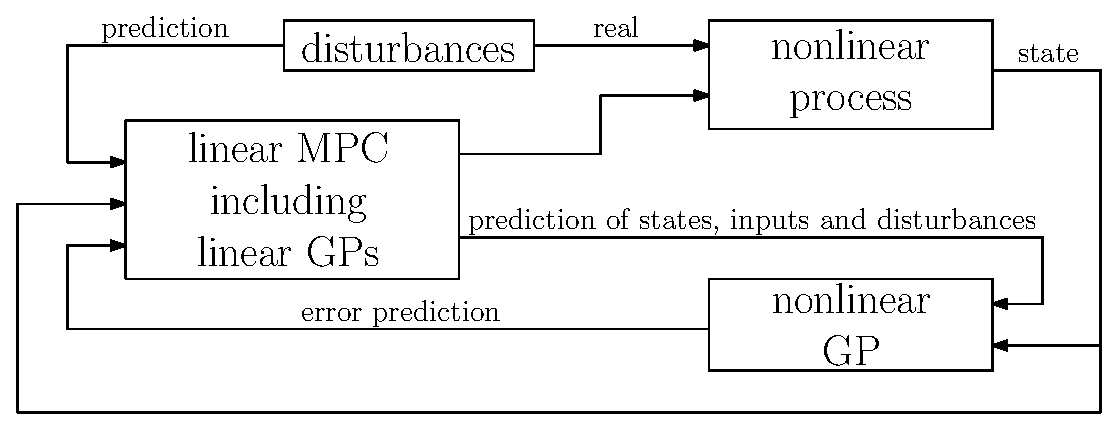
\includegraphics[width=\textwidth]{../Figures/concept_controller.eps}
	\caption{Concept of the augmented MPC}
	\label{fig:concept_controller}
\end{center}
\end{figure}

The full augmented MPC description is given by:
\begin{subequations}\label{eq:description_aug}
\begin{align}
\min \, &J(\mathbf{x},\mathbf{u};\mathbf{d},\mathbf{w})
\end{align}
subject to:
\begin{align}
\dot{\mathbf{x}}_{aug} = A \left( \mathbf{d} \right) \mathbf{x} &+ B \left( \mathbf{d} \right) \mathbf{u} + C \left( \mathbf{d} \right) + \mathbf{w},\label{eq:aug_dyn}\\
\mathbf{x} &\in \mathcal{X}, \mathbf{u} \in \mathcal{U},\label{eq:aug_sets}
\end{align}
\end{subequations}
and the optimal input trajectory $\mathbf{u}^*$ is obtained by:
\begin{align}
\mathbf{u}^* = \underset{\mathbf{u}}{\arg\min}~J(\mathbf{x},\mathbf{u};\mathbf{d},\mathbf{w}), \label{eq:uoptaug}
\end{align}
with respect to the constraints \eqref{eq:aug_dyn} and \eqref{eq:aug_sets}.

%%%%%%%%%%%%%%%%%%%%%%%%%%%%%%%%%%%%%%%%%%%%%%%%%%%%%%%%%%%%%%%%%%%%%%%%%%%%%%%%%%%%%%%%%%%%%%%%%%%%%%%%%%%%%%%%%%%%%%%%%%%%%%%%%%%%%%%%%%%%%%%%%

\section{Prediction model}
\label{sec:predictionmodel}
An analytical linearization of the nonlinear model described in \cref{cha:ICR} was used as the prediction model.
The nonlinear model is denoted as $f_{nl}(\mathbf{x},\mathbf{u};\mathbf{d})$.
The linearization at the point $(\mathbf{x}_0,\mathbf{u}_0)$ is described by:
\begin{align}
\begin{split}\label{eq:linearization}
f_{lin}(\mathbf{x},\mathbf{u};\mathbf{d}) &= f_{nl}(\mathbf{x}_0,\mathbf{u}_0;d)\\
                                          &+ \frac{\partial f_{nl}(\mathbf{x},\mathbf{u};\mathbf{d})}{\partial x} \bigg \vert_{\mathbf{x}_0,\mathbf{u}_0} \cdot (\mathbf{x} - \mathbf{x}_0)\\
                                          &+ \frac{\partial f_{nl}(\mathbf{x},\mathbf{u};\mathbf{d})}{\partial u} \bigg \vert_{\mathbf{x}_0,\mathbf{u}_0} \cdot (\mathbf{u} - \mathbf{u}_0).
\end{split}
\end{align}
\ref{eq:linearization} can also be expressed as a parameter-dependent state-space model \ref{eq:xdotlin}.
The parameters for the linearization are given in \cref{sec:lin_params}.

The linearisation is still parameter-dependent because of the bilinear properties of $f_{nl}(\mathbf{x}_0,\mathbf{u}_0;d)$.
Examining a simplified version of \ref{eq:beta}, described by:
\begin{equation}\label{eq:simple_rs}
Q_{rs,sim} = D_{rs,e}\cdot\left(1-U_{shd}\right),
\end{equation}
we can see that the magnitude of the effect of the shades $U_{shd}$ is heavily depending on the solar radiation $D_{rs,e}$. At night ($D_{rs,e} = 0$) the shades have no effect while at noon ($D_{rs,e} \approx \unit{800}{\nicefrac{W}{m^2}}$) they may be the only way to avoid too high temperatures. This is also the reason why prediction models derived from step and impulse responses perform badly when the environmental variables differ from the test scenario.

Another aspect of our prediction model is the error prediction with GPs.
Taking every variable into account would result in an input space with eleven dimensions.
To reduce the size of the GP identifying the major error sources is necessary.
The wind speed has a major effect on the greenhouse inside air temperature. Hence, establishing a GP for the wind speed $D_{ws,e}$ which is bilinearly and nonlinearly affected with opening percentage of the vents $U_{ven}$ results in an huge improvement of the linear model as \cref{cha:setpoint} will show.

\cref{fig:gp_optimization} shows the GP of the error of the temperature ODE.
Before the optimization of the hyperparameters the error seems arbitrary.
After the optimization a clear pattern is identifiable.
The greater the wind speed and the vents opening the greater the error.
Since the system is linearized around $(U_{ven} = 0.1, D_{ws,e} = 0)$ the error growth in dependence of the distance to this point seems valid.

% \begin{figure}[t]
% \begin{center}
% 	\begin{subfigure}[t]{.49\textwidth}
% 	\centering
% 		\includegraphics[width=\textwidth]{../Figures/gp_plot_not_opt.eps}
% 		\caption{Before optimization}
% 		\label{fig:gp_before_opt}
% 	\end{subfigure}
% 	\hfill
% 	%\newline
% 	\begin{subfigure}[t]{.49\textwidth}
% 	\centering
% 		\includegraphics[width=\textwidth]{../Figures/gp_plot_opt.eps}
% 		\caption{After optimization}
% 		\label{fig:gp_after_opt}
% 	\end{subfigure}
% \caption{GP describing the error for the temperature ODE caused by the linearization in dependence of $U_{ven}$ and $D_{ws}$}
% \label{fig:gp_optimization}
% \end{center}
% \end{figure}

%%%%%%%%%%%%%%%%%%%%%%%%%%%%%%%%%%%%%%%%%%%%%%%%%%%%%%%%%%%%%%%%%%%%%%%%%%%%%%%%%%%%%%%%%%%%%%%%%%%%%%%%%%%%%%%%%%%%%%%%%%%%%%%%%%%%%%%%%%%%%%%%%

\section{Software}
\label{sec:software}

The MPC was implemented via the use of several frameworks for Python 2.7.
\textbf{do-mpc} \cite{Lucia.2017}, a nonlinear MPC framework with integrated optimization, is the central element.
It consists of four modules: model, optimizer, observer and simulator.
Due to this modularity switching between different setups, e.g. changing the prediction model, is simple and analysis is simplified.

For the optimization tasks \textbf{Ipopt} \cite{Wachter.2006} is employed.
It is a primal-dual interior-point algorithm with a filter line-search method for nonlinear programming including second order corrections.
\textbf{CasADi} \cite{Andersson.01.01.2013} is a symbolic software tool for automatic differentiation and dynamic optimization used for the modeling and for the computation of first and second order derivative information.
\textbf{GPy} \cite{GPy.since2012} is the Gaussian process framework utilized for the augmented MPC. It includes a multitude of models, kernels and likelihoods for modelling stochastic processes and computing their optimal parameters.
\cref{fig:implementation_software} recaps the relations between the single software tools.
The module observer is not mentioned explicitly because full state feedback was used.\par\medskip

\begin{figure}[t]
\begin{center}
	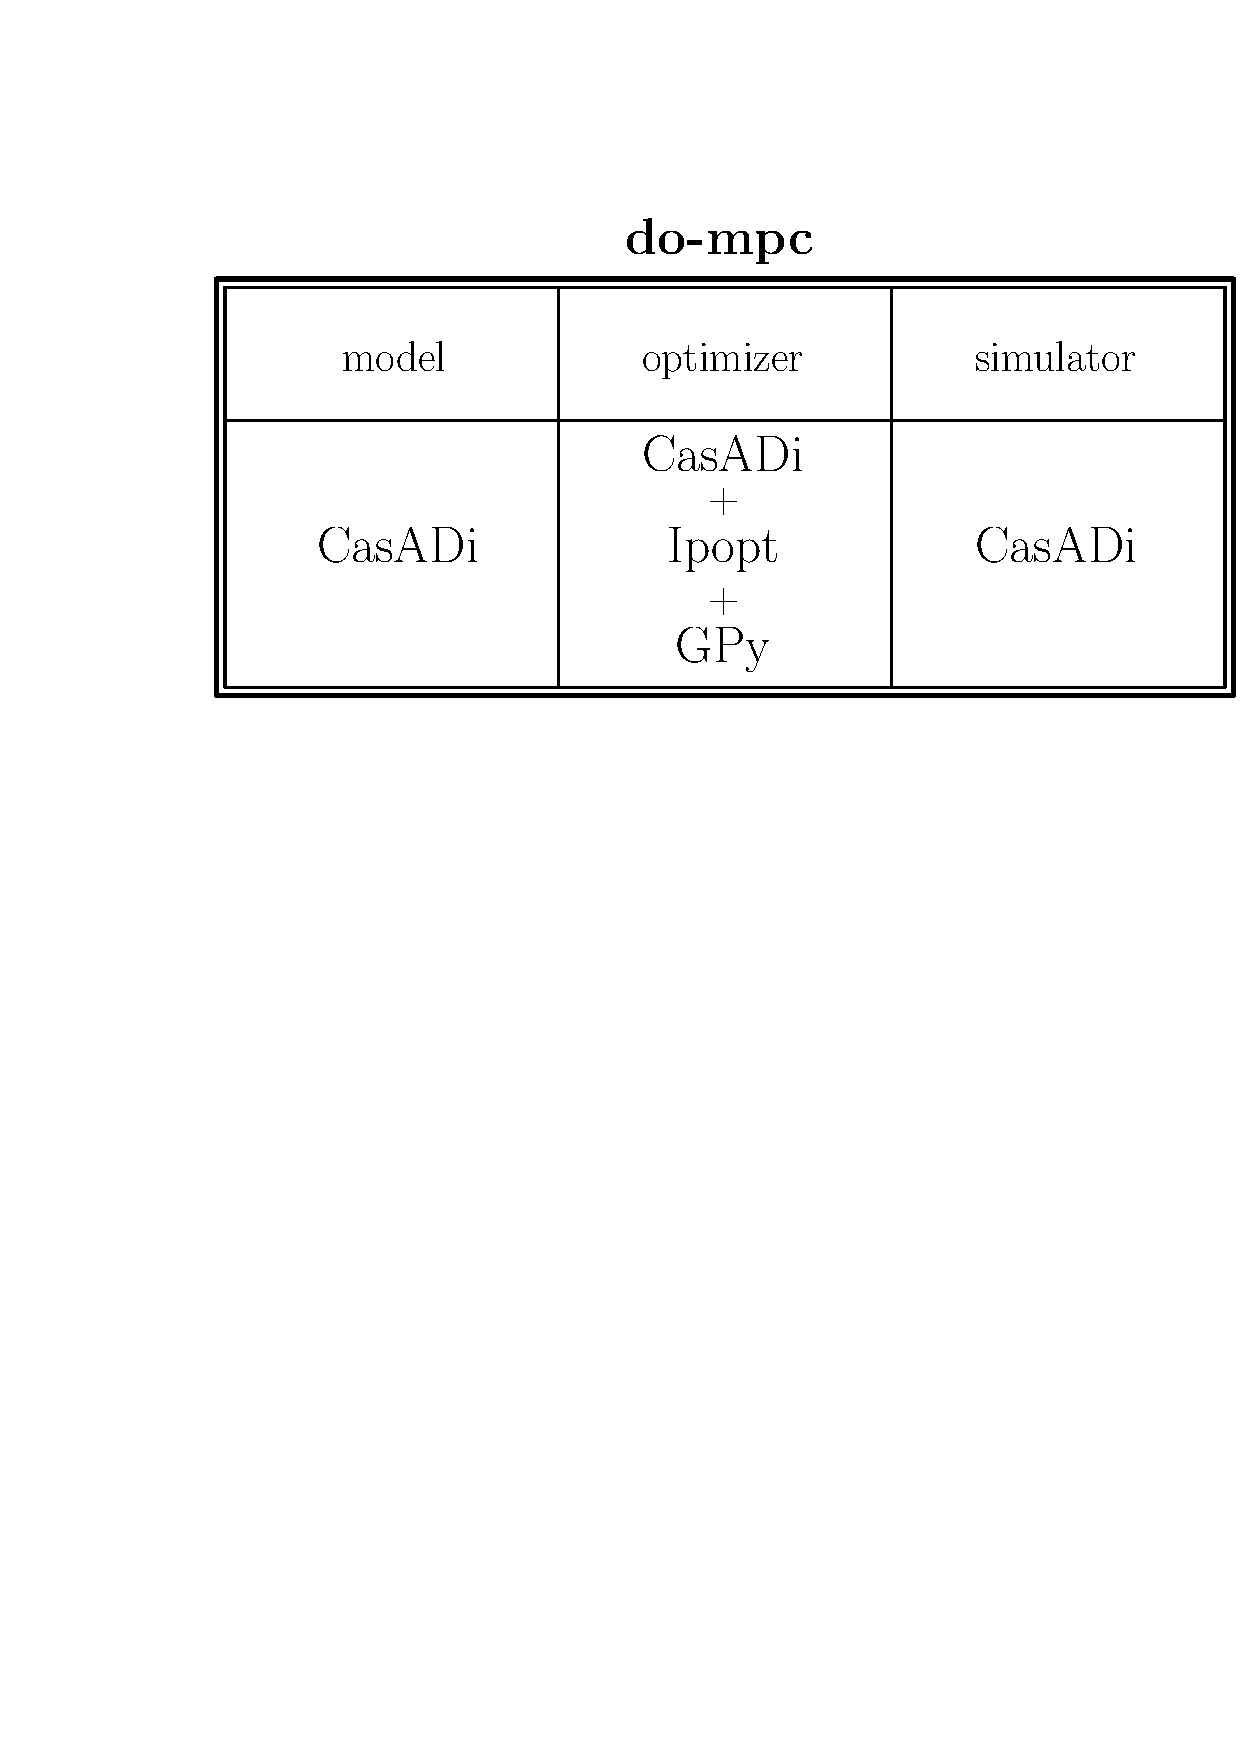
\includegraphics[width=\textwidth]{../Figures/implementation_software.pdf}
	\caption{Relations between the software tools}
	\label{fig:implementation_software}
\end{center}
\end{figure}

In summary, this chapter illustrated the concept of the expanded MPC approach.
Moreover, the linear prediction model used for the approach was derived and the software tools to implement the new concept were described.
In the following two chapters the newly derived augmented MPC scheme is used for set-point tracking (\cref{cha:setpoint}) and economic MPC (\cref{cha:economic}).